\newpage
\section{Resultados}

\subsection{Calculo do indutor}

Para o calculo do indutor, foi utilizada a equação \ref{e_freq}, sendo re-escrita de modo a obter o valor de L (equação (\ref{equ:L})).

\begin{equation}
    \label{equ:L}
    L = \frac{1}{(2\pi f_0)^2 C}.
\end{equation}

Através da inspeção do circuito, o valor de $C$ em (\ref{equ:L}) é:
\begin{equation}
    \label{equ:C}
    C = \frac{C_1 C_2}{C_1 + C_2}.
\end{equation}

Substituindo os valores dados em (\ref{equ:L}) e (\ref{equ:C}), temos que $L = 3,5267 \ \mu H$.

Assim, o circuito foi montado no software ORCAD, conforme mostra a figura \ref{fig:cir}.

\begin{figure}[H]
    \centering
    \caption{Circuito a ser analisado no software ORCAD.}\label{fig:cir}
%   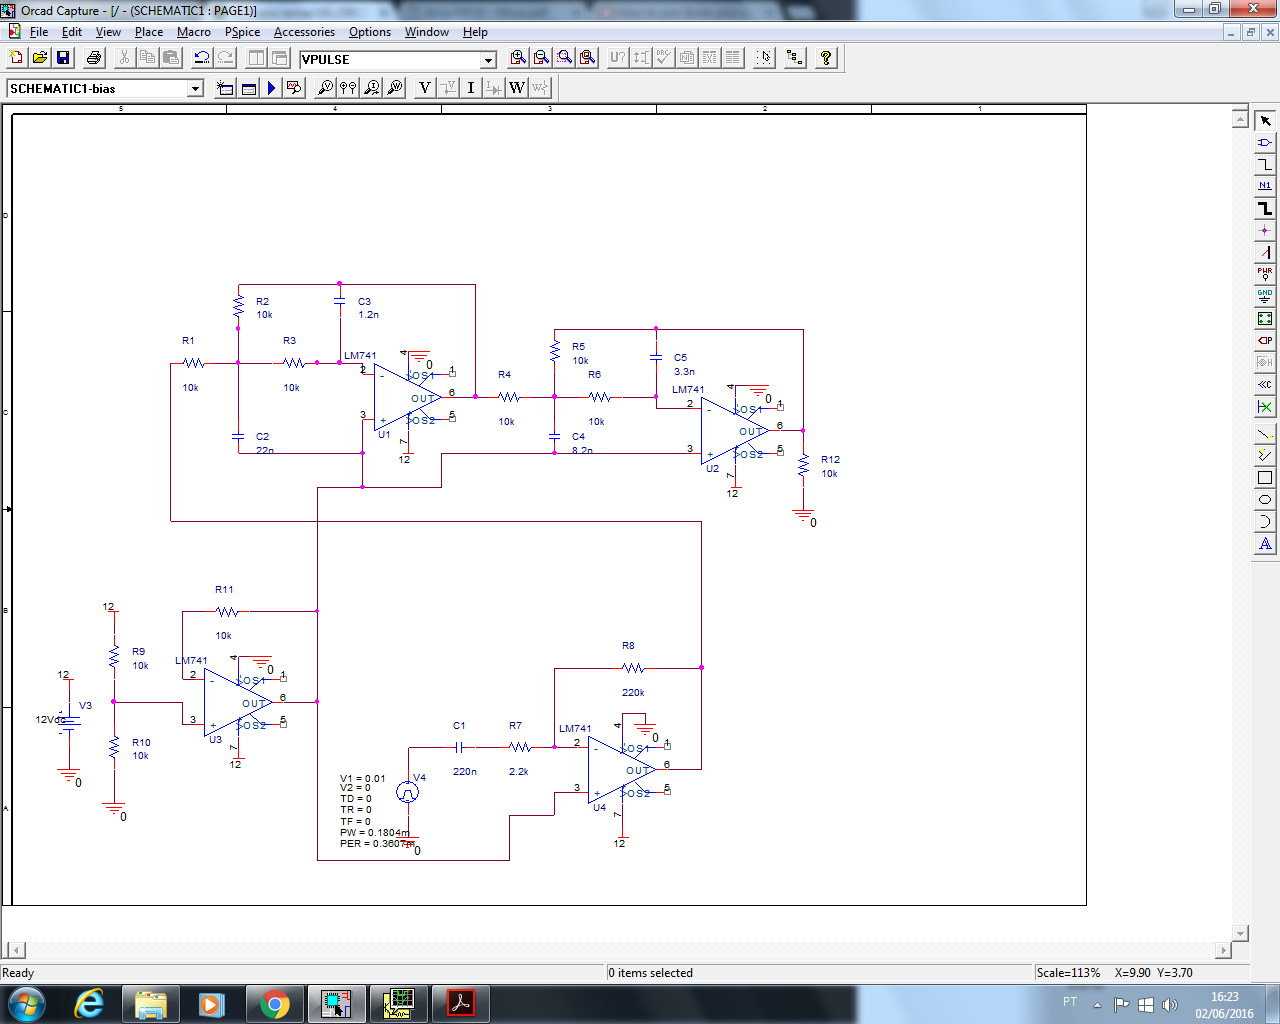
\includegraphics[scale=0.5]{Imagens/cir}

    \small Fonte: Autoria própria.
\end{figure}

\subsection{Simulação do circuito}

Após a simulação do circuito, foi obtida a forma de onda da figura \ref{fig:out}, onde apresenta uma senoide de frequência $4,17 \ [MHz]$, e uma tensão de pico a pico de $V_{pp} = 769,06 \ [mV]$. Nota-se que o valor da frequência obtida experimentalmente é bastante próximo do valor teórico ($4 \ [MHz]$).

\begin{figure}[H]
    \centering
    \caption{Sinal na saída do circuito.}\label{fig:out}
    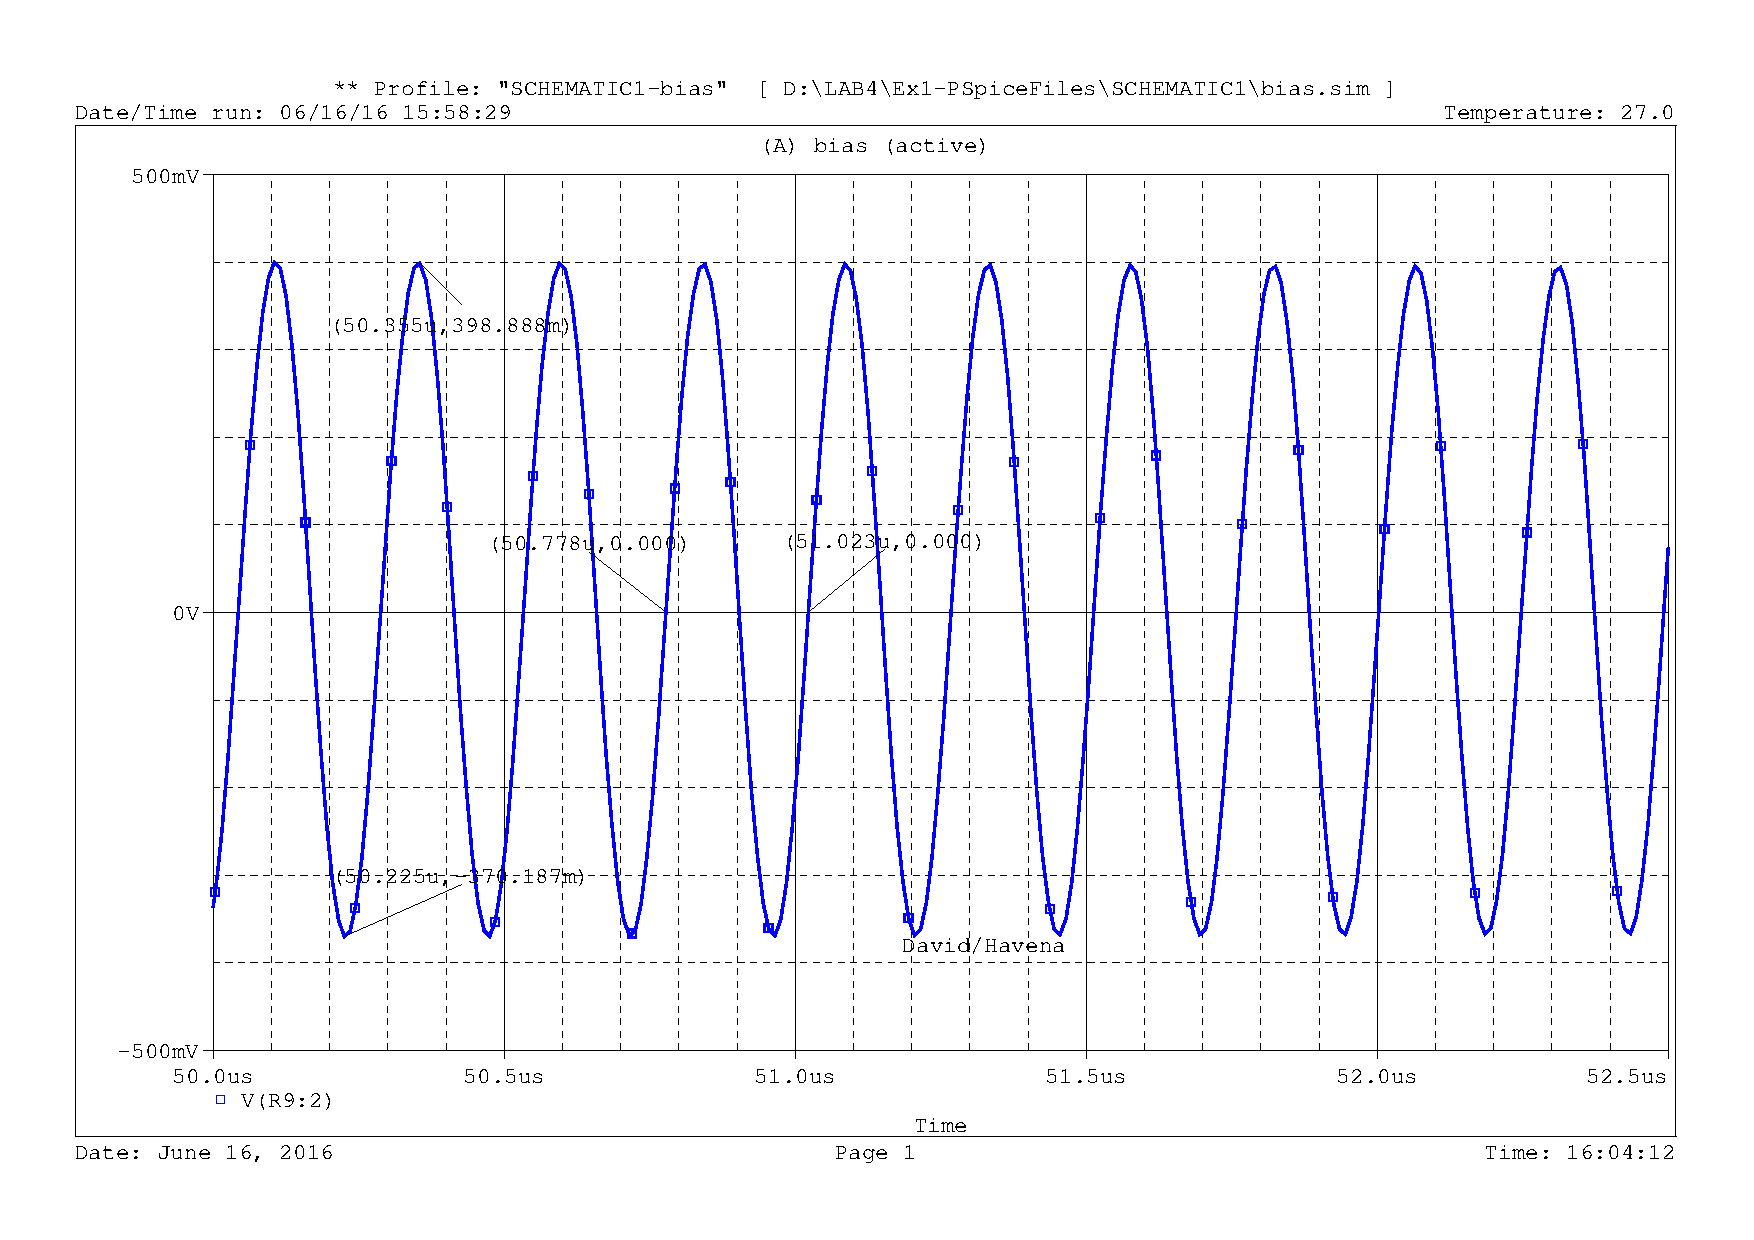
\includegraphics[scale=0.5]{Imagens/out}
    
    \small Fonte: Autoria própria.
\end{figure}

Também foi obtido o sinal na saída do oscilador, conforme mostra a figura \ref{fig:osc}. Os valores notáveis estão apontados no gráfico.

\begin{figure}[H]
    \centering
    \caption{Sinal na saída do oscilador.}\label{fig:osc}
    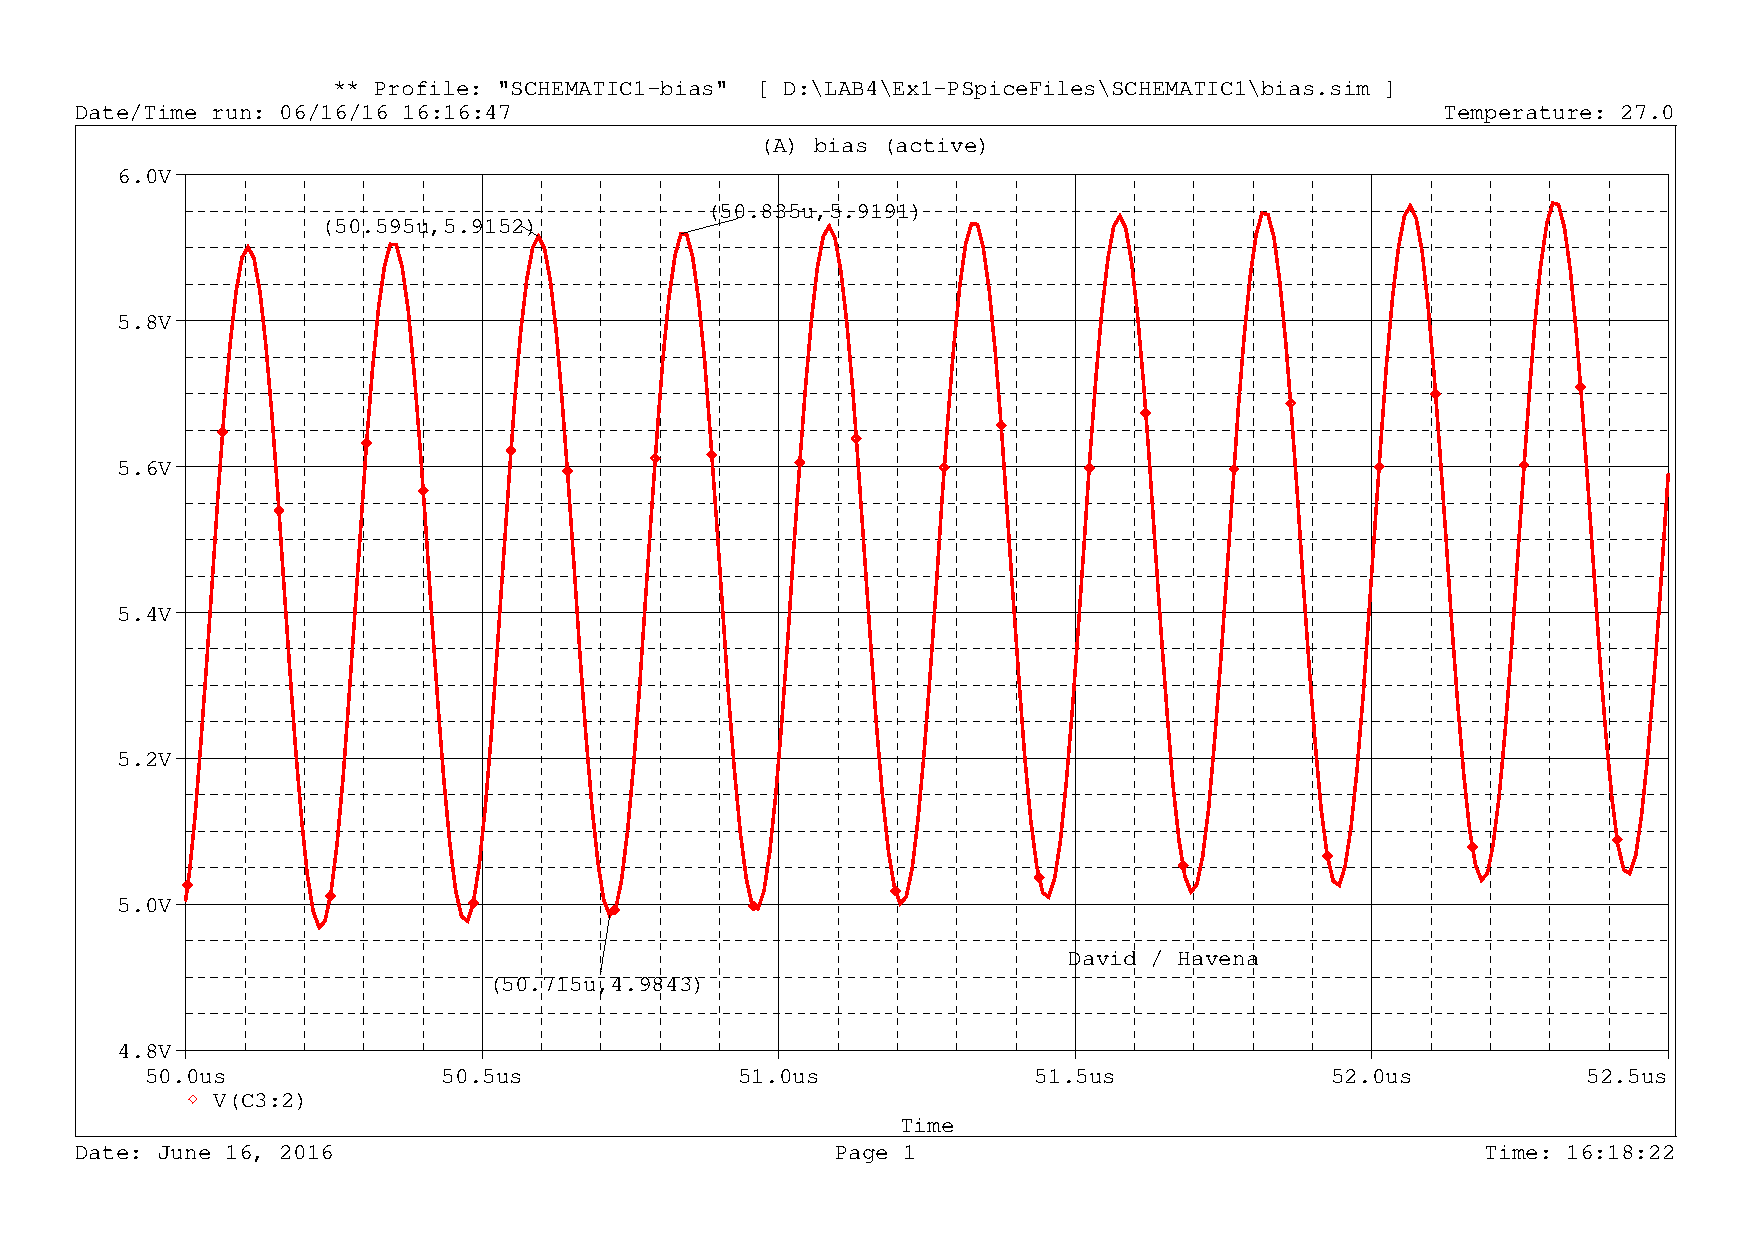
\includegraphics[scale=0.5]{Imagens/osc}
    
    \small Fonte: Autoria própria.
\end{figure}

\subsection{Interferência da ponta de prova de um osciloscópio}
Para simulação da ponta de prova de um osciloscópio, foi utilizado um circuito composto de um capacitor de $50 \ pF$ e um resistor de $10 \ M\Omega$ em paralelo aos pontos de teste.

Os valores para da alteração na frequência de saída e tensão de pico a pico para cada um dos pontos são apresentados na tabela \ref{tab:pontadeprova}. Foi observado que o maior desvio na frequência de saída ocorre quando a ponteira está em paralelo com o o capacito $C_1$.

\begin{table}[H]
    \begin{center}
        \caption{Tensão de saída e frequência para o circuito com a ponta de prova em determinados pontos}\label{tab:pontadeprova}
        \begin{tabular}{ccc}
            \hline
            Local & Frequência de saída [MHz] & $V_{pp}$ [mV]\\
            \hline
             Saída do oscilador& 4,115 & 813,353 \\
             Coletor de Q1 & 4,048 & 817,73\\
             J1 & 4,098 & 812,906\\
             Sobre $C_1$ & 4,048 & 823,109 \\
            \hline
        \end{tabular}
        
        \small Fonte: Autoria Própria.
    \end{center}
\end{table}

\subsection{Distorção Harmônica}

As figuras \ref{fig:fftout} e \ref{fig:fftosc} mostram o espectro dos sinais na saída do circuito e na saída do oscilador respectivamente. É possível observar que o conteúdo espectral da segunda e terceira harmônica, em ambos os casos, possui baixa quantidade de energia.

\begin{figure}[H]
    \centering
    \caption{Espectro do sinal na saída do oscilador.}\label{fig:fftout}
    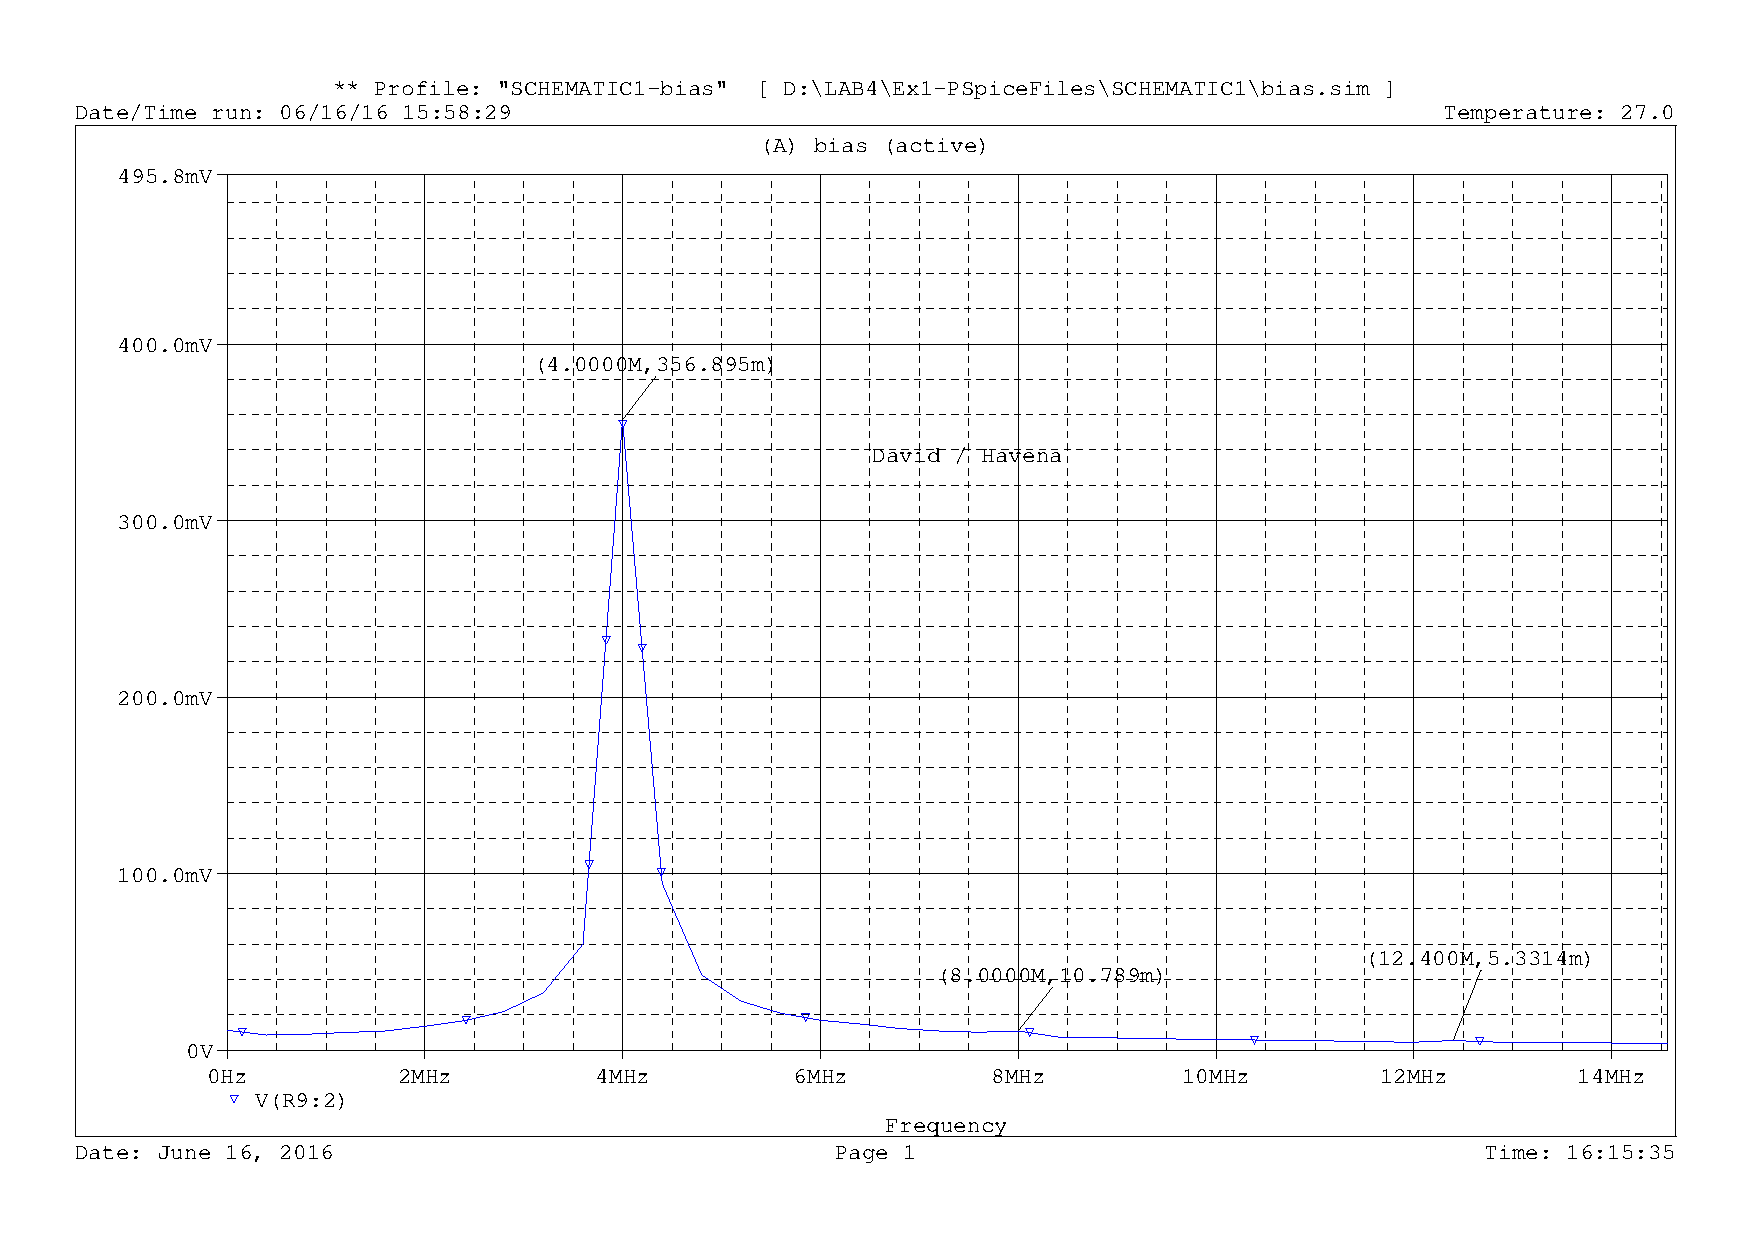
\includegraphics[scale=0.5]{Imagens/fftout}
    
    \small Fonte: Autoria própria.
\end{figure}

Na figura \ref{fig:fftosc} nota-se que existe grande quantidade de energia no nível DC, porém, essa componente é filtrada antes da saída do circuito.

\begin{figure}[H]
    \centering
    \caption{Espectro do sinal na saída do oscilador.}\label{fig:fftosc}
    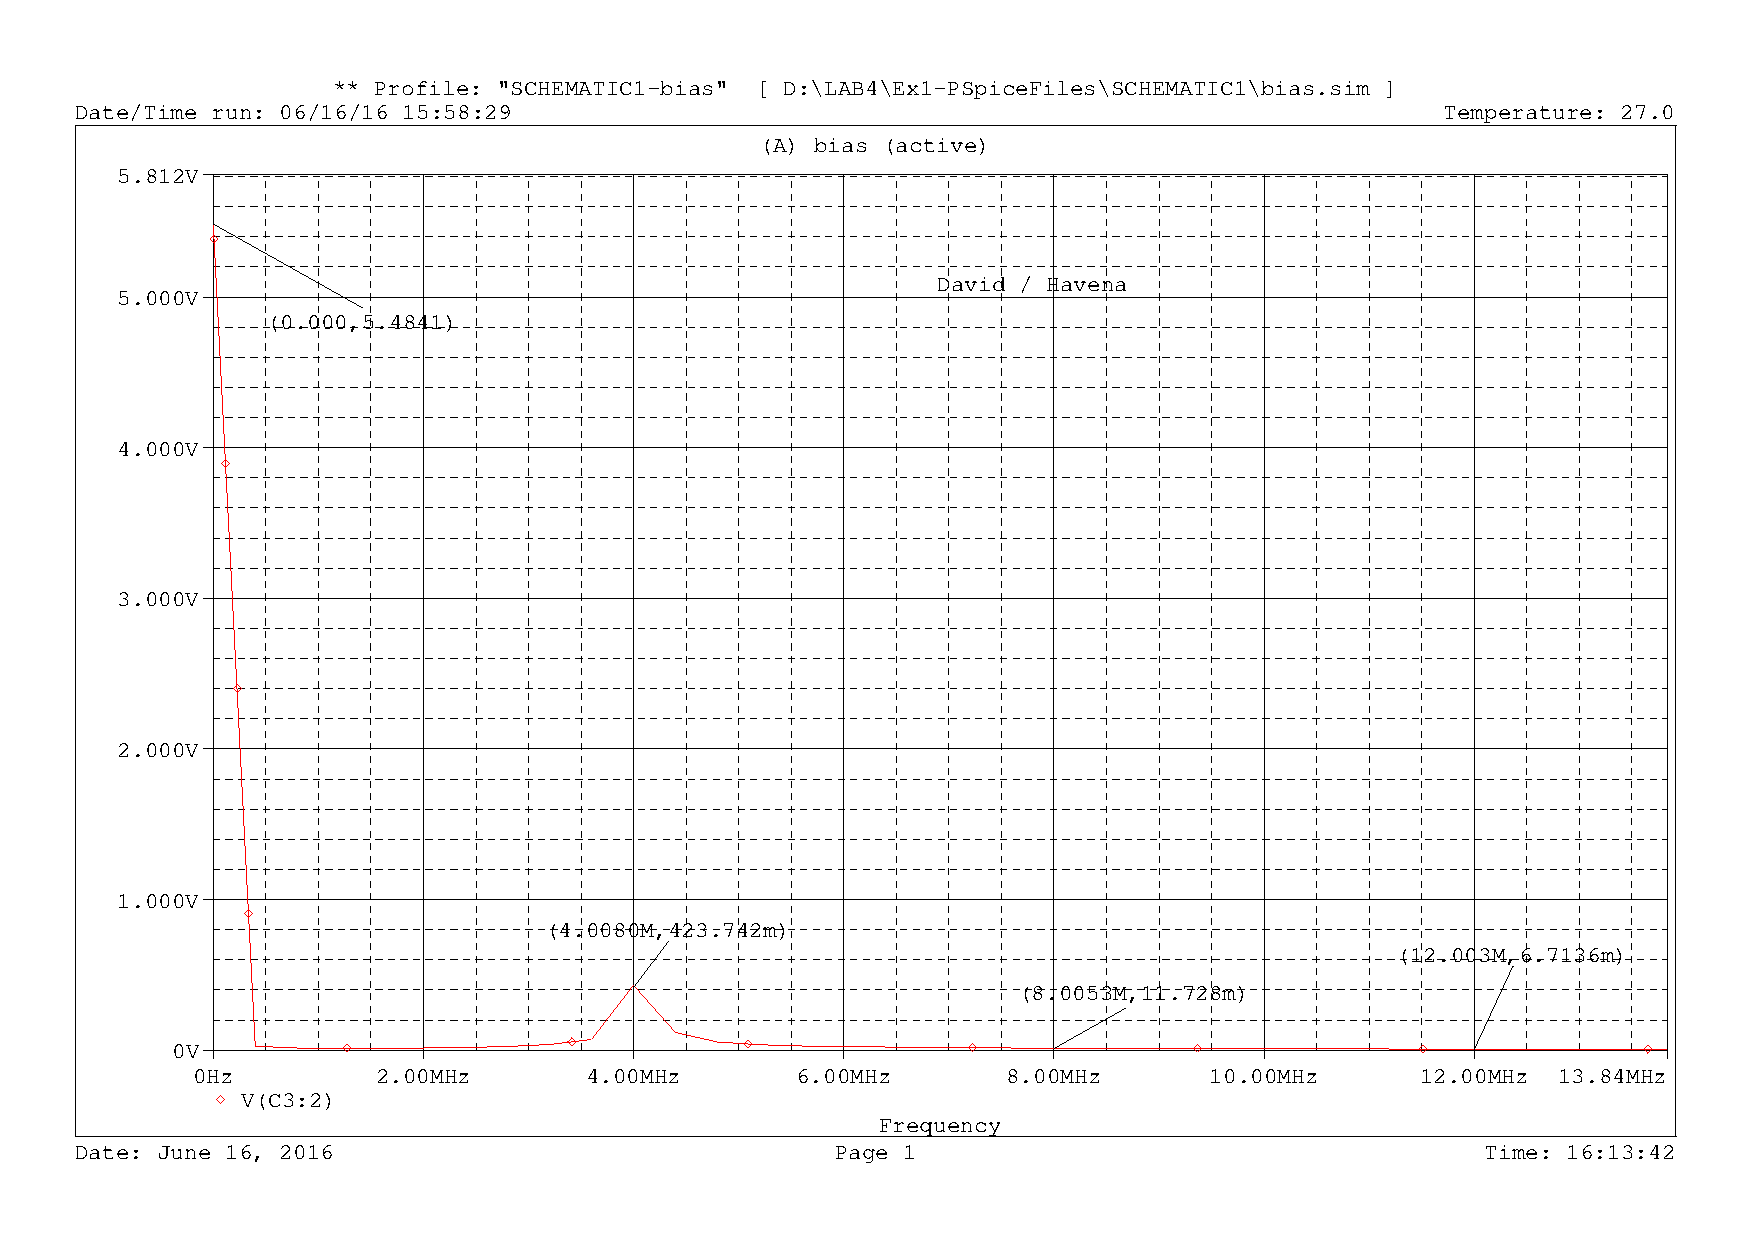
\includegraphics[scale=0.5]{Imagens/fftosc}
    
    \small Fonte: Autoria própria.
\end{figure}

A tabela \ref{tab:distor} sumariza os valores de energia para a primeira e segunda harmônica da saída do circuito.

\begin{table}[H]
    \begin{center}
        \caption{Potência RMS para as componentes espectrais do sinal de saída.}\label{tab:distor}
        \begin{tabular}{cc}
            \hline
            Componente & Potência \\
            \hline
            Fundamental & $2,548 \ mW$ \\
            Primeira Harmônica & $2,32 \  \mu W$ \\
            Segunda Harmônica & $0,568 \ \mu W$\\
            \hline
        \end{tabular}
        
        \small Fonte: Autoria Própria.
    \end{center}
\end{table}

\subsection{Estabilidade do circuito}

Para analisar a estabilidade, o circuito foi simulado com a fonte de alimentação em 9,6 V e, em seguida, 14,4 V. A frequência de saída obtida para os 2 valores de tensão foram:

\[
    f_{9,6V} = 4,115 \ [MHz],
\]

\[
    f_{14,4V} = 4,098 \ [MHz].
\]

O desvio de frequência em partes por milhão por volts foi calculado como sendo:

\[
    \left[\frac{\Delta f / f}{V}\right] = \frac{4,115 - 4,098}{(14,4-9,6)4,08} = 868,05 \ \left[\frac{Hz/MHz}{V}\right]
\]

O valor obtido demonstra que o circuito é bastante estável em relação a variações na tensão de alimentação do circuito.